\chapter{Separace budicího a odraženého signálu}
Pro potřeby zpracování změřených dat je nezbytné separovat budicí signál od jeho odrazů. Takovou separaci je možné provádět buď hardwarově v době měření nebo až během zpracování změřených dat. Cílem je dosáhnout toho, aby byly tyto dva signály zcela oddělené (či oddělitelné při zpracování). Možné metody separace:
\begin{itemize}
	\item
	\textbf{Směrová odbočnice}\\*	
	\begin{figure}[htbp]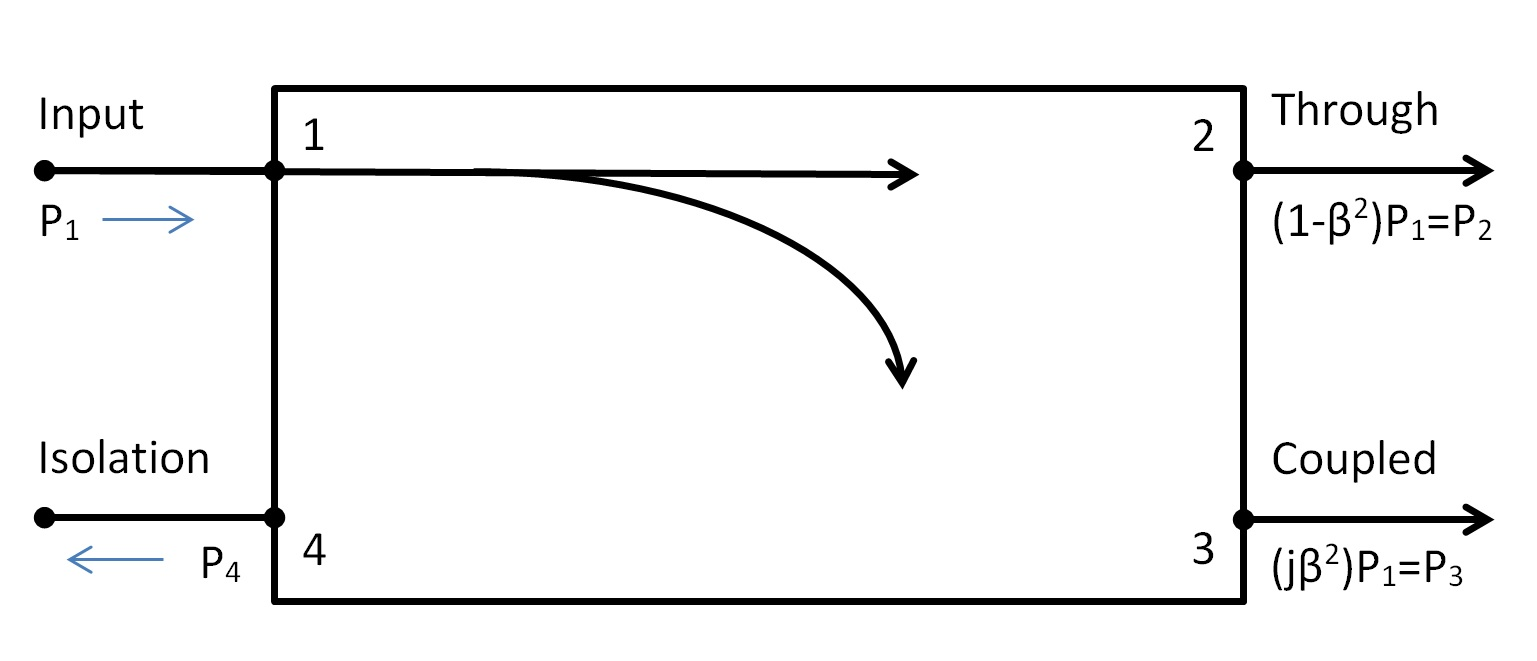
\includegraphics[width=.8\textwidth,keepaspectratio]{images/directionalcoupler.png}\caption{Směrová odbočnice, převzato z \cite{widebandcouplers}.}\label{directionalcoupler}\end{figure}	

	Pomocí tradičních odbočnic jako na obr. \ref{directionalcoupler} je možné provádět separaci s velkou izolací nechtěného signálu, ovšem nesplňují požadavek na šířku zpracovávaného pásma \cite{widebandcouplers}. Problematická je také skutečnost, že s rostoucí šířkou použitelného pásma odbočnice obvykle klesá směrovost odbočnice. Dochází tedy pouze k částečné separaci, další separační krok by byl nezbytný během zpracování naměřených dat.
	
	\item
	\textbf{Odporový můstek}\\*	
	\begin{figure}[htbp]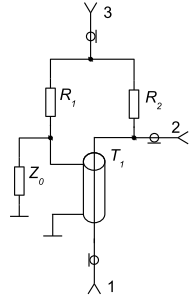
\includegraphics[width=\textwidth,height=5cm,keepaspectratio]{images/resistivebridge.png}\caption{Odporový směrový můstek, převzato z \cite{resistivedirectionalbridge}.}\label{resistivebridge}\end{figure}	
	Pomocí odporových můstků je možné provádět separaci signálů s velmi velkou šířkou pásma, např. v \cite{resistivedirectionalbridge} a obr. \ref{resistivebridge} uveden můstek pro pásmo \SI{300}{\kilo\hertz}--\SI{13.5}{\giga\hertz}. Opět ovšem nejsou signály plně separovány, je nezbytný další separační krok během zpracování.
	
	\item
	\textbf{Časové oddělení}\\*	
	Pokud má budicí signál tu vlastnost, že má omezenou délku, po kterou se mění a mimo ni je konstantní (vybraný jednotkový skok tuto vlastnost splňuje), je možné jej od odrazů separovat tak, že je časově posunut vůči odezvě systému. Toho je možné dosáhnout například použitím dokonalého vedení bez odrazů, které se zapojí mezi bod měření a měřený systém. Jeho délka musí být minimálně taková, aby se nemohla nikdy překrývat nekonstantní část budicího signálu s odrazy. Pokud je v naměřených datech známá poloha budicího pulzu (nebo je-li možné jej spolehlivě identifikovat), je možné naměřená data rozdělit na část buzení a část odpovědi měřeného systému. První část pak může sloužit ke korekci frekvenční charakteristiky změřené odezvy systému a odhadu šumového spektra. Známe-li i přesnou délku prodlužovacího vedení (hrubě z návrhu zařízení, přesně pomocí kalibrace), je možné provést kalibraci měřicí roviny. Při použití této metody separace stačí vzorkování pouze jednoho průběhu, snižuje tedy počet potřebných vzorkovačů ze dvou (nebo více) na jeden. Z toho také vyplývá, že měřená data nejsou zatížena chybou, která by mohla vzniknout vzhledem k rozdílným vlastnostem jednotlivých vzorkovačů.
	
	Na obrázku \ref{separableunitstep} je znázorněna odezva na chybovou funkci. Buzení se nachází v čase $t=0$, odezva v čase $t=0.5$. Průběh budicí funkce je předem známý, nekonstantní část průběhu se nepřekrývá s odezvou, je tedy možné je v časové oblasti $t\in (0;0.5)$ rozdělit na dva samostatné průběhy.

\begin{figure}[htbp]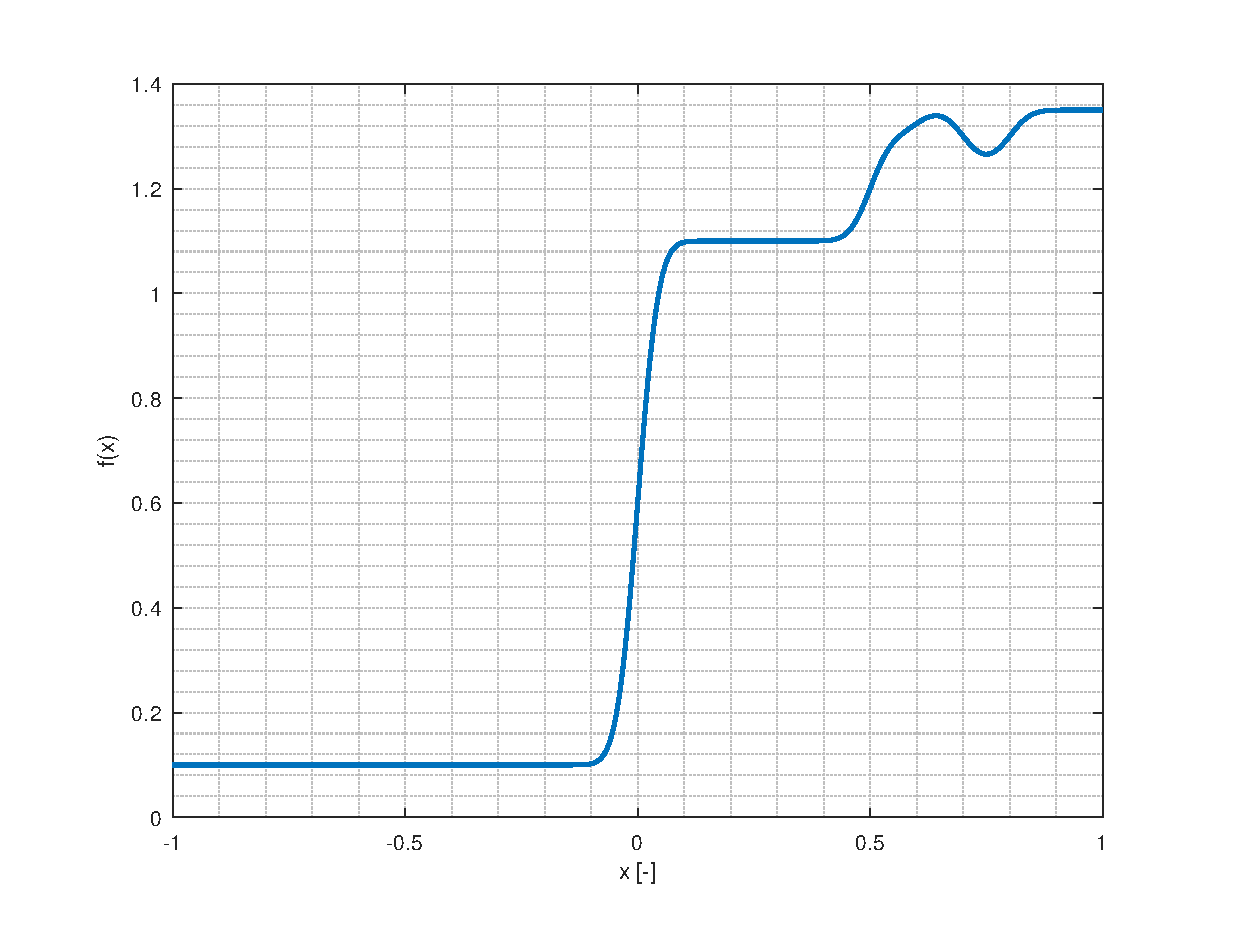
\includegraphics[width=\textwidth,keepaspectratio]{images/separableunitstep.eps}\caption{Časově oddělitelná odezva na jednotkový skok.}\label{separableunitstep}\end{figure}	
\end{itemize}

Pro vybraný budicí signál (jednotkový skok) je tedy možné provést separaci od odrazů zpožďovacím vedením a vhodným rozdělením naměřených dat na dvě části. Toto řešení se jeví jako obvodově i výpočetně nejjednodušší z uvažovaných metod separace.